\documentclass{article}

% use Times
\usepackage{times}
% For figures
\usepackage{graphicx} % more modern
%\usepackage{epsfig} % less modern
\usepackage{subfigure}

% For citations
\usepackage{natbib}

% For algorithms
\usepackage{algorithm}
\usepackage{algorithmic}

% As of 2011, we use the hyperref package to produce hyperlinks in the
% resulting PDF.  If this breaks your system, please commend out the
% following usepackage line and replace \usepackage{icml2015} with
% \usepackage[nohyperref]{icml2015} above.
\usepackage{hyperref}

% Packages hyperref and algorithmic misbehave sometimes.  We can fix
% this with the following command.
\newcommand{\theHalgorithm}{\arabic{algorithm}}

% Employ the following version of the ``usepackage'' statement for
% submitting the draft version of the paper for review.  This will set
% the note in the first column to ``Under review.  Do not distribute.''
%\usepackage{icml2015}

% Employ this version of the ``usepackage'' statement after the paper has
% been accepted, when creating the final version.  This will set the
% note in the first column to ``Proceedings of the...''
\usepackage[accepted]{icml2016}

\begin{document}

\twocolumn[
\icmltitle{Gesture Recognition with Batch and Reinforcement Learning}

% It is OKAY to include author information, even for blind
% submissions: the style file will automatically remove it for you
% unless you've provided the [accepted] option to the icml2015
% package.
\icmlauthor{Andrew Ciambrone}{andrjc4@vt.edu}
\icmlauthor{Arpit Goyal}{arpitg@vt.edu}
\icmlauthor{Hossameldin Shahin}{hshahin@cs.vt.edu}

\vskip 0.3in
]

\begin{abstract}
Designing an application for recognition of user-defined hand gestures captured via a web camera. The user trains the system for 5-8 distinct hand gestures (training phase). Then, the system predicts the user’s gestures (testing phase). For each wrong prediction, the system retrains itself for better accuracy.
\end{abstract}

\section{Introduction}
\label{Intro}
%% Not actually keeping the subsections just keeping a layout
\subsection{Motivation}
% COMMENT OUT INSTEAD OF DELETING THERE IS NO HISTORY ON OVERLEAF
A Natural user interface, or NUI, is a type of user interfaces that use a user’s natural abilities such as speech or their own movement to interact with a system. It is believed by many that NUI's will revolutionize the way a user interacts with a system because this type of interface is invisible to the user. One common method of interaction is using hand gestures. By using gesture recognition, a user can interact with a system more efficiently and intuitively.
\subsection{Problem}
Gesture recognition is a problem of classification. A gesture recognition system must be able to read in inputs and output the correct gesture. Because gesture recognition typically uses a camera to observe the gestures this problem falls into the fields of computer vision for data extraction and machine learning for classification. Capturing the hand gesture is an complex\
\subsection{Approach}
Approach: The problem statement can be broken down into the following subparts:
Feature extraction: We do a set of operations on the input video feed to remove the background clutter and get a binary image with only user's hand in the foreground. This includes background subtraction, thresholding, skin color detection, finding biggest contour etc. We can use a modified version of 1 algorithm for scale-and-rotation invariance. For rotation invariance, the indicative angle (the angle between the centroid and the first contour point of the gesture) is calculated. The gesture is rotated until this angle goes to zero. For scale-invariance, the gesture is scaled to a standard square. We can then use the coordinates of the contour points and that of the centroid as features to train our supervised learning model. We also extract the convex hull points and convexity defects in the hand contour and filter out irrelevant defects and vertices, thresholding on the angle made by two vertices and a defect point. We add the number of vertices and defect points, minimum/maximum/sum of the distances of vertex points from the centroid, etc. to the feature space.
Model training: A supervised learning model, like a multi-class Support Vector Machine (SVM) (experiment with linear/polynomial/RBF kernels) or a Neural Network (experiment with varied number of layers and hidden units) is used to train on the user's input gestures in the feature space described above. We use 'n' (20-30) images for each gesture. We save the learned model parameters for each gesture.
Gesture recognition: In the testing phase, we extract the above features for each frame in the input video feed. We calculate the probability of each trained gesture matching the input gesture using our trained SVM model. If the maximum probability exceeds a minimum threshold, we store the gesture ID, input features and the probability value for this frame. We can also use the difference between the highest probability gesture and the second highest probability gesture as a measure of confidence for the prediction, and put a threshold on this confidence value.
Reinforcement learning: For the system to better itself over time, we deploy a reinforcement learning model (say q-learning), where the user can give his negative feedback for a wrong prediction by hitting the spacebar on the computer. The model pays a penalty for each wrong prediction by reducing from the weight vector of the last predicted class. We can experiment with various Markov chain lengths to see which performs the best for our use-case. During the reinforcement learning phase we will also start simple with the gesture data. With a plain background and as the accuracy increases move up to more complex gesture data. Our hope is that by starting off simple the algorithm can train itself  so that it can handle more complex models as the gesture images become more complex.

\section{Related Work}

\section{Technical Contribution}

\subsection{System}

\subsubsection{Computer Vision}
\subsubsection{Training}
\subsubsection{Reinforcement Learning}


\subsection{Data Used}
%---------------------------------------------------------------------------%
% 							Begin: Hossam									%
% --------------------------------------------------------------------------%

% ***** table: best parameter values ---> move up to make it in the correct page*****
\begin{table*}[t]  % table spans two columns
% \begin{table}[t]  	% table uses one column
\caption{Best chosen parameters for each model.}
\label{tab:bestParams}
\vskip 0.15in
\begin{center}\begin{small}\begin{sc}
  \begin{tabular}{lccccccccccr}
    \hline
    \abovespace\belowspace
    Number of &  \shortstack{a\\b} &  &  &  &  &  &  &  &  &  \\
    \hline
    Gestures  &\multicolumn{1}{|p{1.0cm}}{\centering kernel}
              &\multicolumn{1}{p{0.5cm}}{\centering C}
              &\multicolumn{1}{p{1.0cm}}{\centering degree}
              &\multicolumn{1}{p{1.0cm}}{\centering gamma}
              &\multicolumn{1}{|p{1.0cm}}{\centering splitter}
              &\multicolumn{1}{p{1.25cm}}{\centering max depth}
              &\multicolumn{1}{|p{0.75cm}}{\centering alpha}
              &\multicolumn{1}{p{1.5cm}}{\centering hidden \\ layers \\Size}
              &\multicolumn{1}{|p{1.25cm}}{\centering max \\ depth}
              &\multicolumn{1}{p{1.25cm}}{\centering n \\ estimators} \\
    \hline
    \abovespace\belowspace
    5         &\multicolumn{1}{|c}{poly}
              &0.72
              &4
              &51.80
              &\multicolumn{1}{|c}{best}
              &26
              &\multicolumn{1}{|c}{0.14}
              &25,27
              &\multicolumn{1}{|c}{20}
              &22  \\
    \abovespace\belowspace
    10        &\multicolumn{1}{|c}{poly}
              &0.02
              &4
              &6.25
              &\multicolumn{1}{|c}{best}
              &17
              &\multicolumn{1}{|c}{1.67}
              &28,24
              &\multicolumn{1}{|c}{13}
              &10  \\
    \hline
  \end{tabular}
\end{sc}\end{small}\end{center}
\vskip -0.1in
\end{table*}
% \end{table}


\section{Hand Gesture Model Selection}

\subsection{Classification Models}

Four machine learning models were considered for the classification of hand gestures, namely: support vector machines (SVM), neural networks, decision trees, and random forest. We used examined three kernels for the SVM: radial basis function (RBF), linear and polynomial.
Each model has multiple parameter to optimize that is called hyper-parameters. The SVM has the parameters: Regularization constant C, $\epsilon$ for round-off error, gamma, and the degree of the polynomial for polynomial kernels. The decision tree has the parameters: minimal number of data instances at a leaf node, the pruning strategy, and the split strategy (best, random). For the random forest, in addition to decision tree parameters, we have number of decision trees (n estimators). Finally the neural network has the parameters:
number of hidden layers, number of hidden units, alpha, and the learning rate.

Finding the best model configuration is clearly not trivial since the choice has to be made at run time. In the next section we propose a solution to find the best model in a feasible amount of time.

\subsection{Hyper-parameter Optimization}
%TODO: rewrite into a paragraph
- how to find model parameters
- No configuration is optimal for all problem domains
- exhaustive search
- Hyperparameter optimization is searching the space of possible configuration variables
- Sequential model-based optimization (SMBO), aka Bayesian optimization, is an efficient method for function minimization
- The Hyperopt library provides algorithms and parallelization infrastructure for performing - hyperparameter optimization (model selection) in Python

Can handle hundreds of variables


% -----------------------------------------------------------
\subsection{Results}


\subsubsection{Hyper-parameter Analysis}
To show the difficulty of choosing the best parameters we plot parts of the search space for each model. Noting that since the user will train his own models, it is possible that the best model parameters will differs from the presented best model.

% TODO: paragraph about SVM results

% TODO: paragraph about neural network results
Figure~\ref{fig:DT_dept_split} shows the accuracy of the Decision tree model for split strategies best and random, using different maximum depth. Result is shown for $5$ gestures and $10$ gestures data sets. Maximum depth greater than $15$ produces comparable prediction error. There is no overall best split strategy for larger maximum depth according to Figure~\ref{fig:DT_dept_split}.

Random forest accuracy improves by increasing number of estimators to some extent where the improvement is limited compared to the increased running time. Figure~\ref{fig:randomForest_estimators} shows the prediction error for number of estimators 10, 20, 30 and 40. The effect of maximum depth of the trees within the random forest has a small variable effect after depth of $20$. Choosing a general optimal value for the depth is not possible but a suggested range be from $20$ to $40$.

% ***** SVM  ???*****
% \begin{figure}[th]
% \vskip 0.2in
% \begin{center}
% \centerline{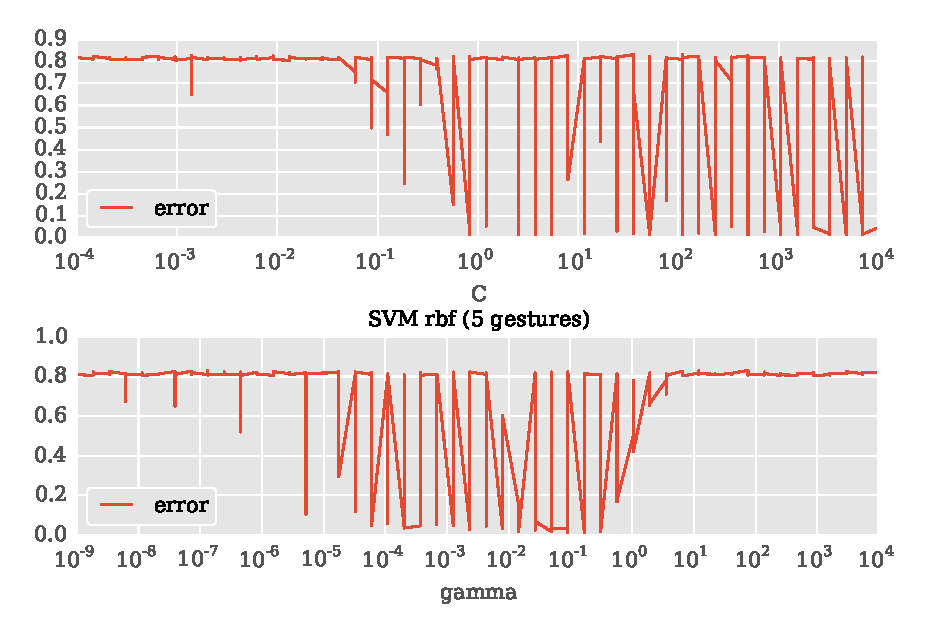
\includegraphics[width=\columnwidth]{svm_C_gamma_5.eps}}
% \caption{SVM (not good).}
% \label{fig:svm}
% \end{center}
% \vskip -0.2in
% \end{figure}

% ***** Neural Network ???*****
% \begin{figure}[th]
% \vskip 0.2in
% \begin{center}
% \centerline{\includegraphics[width=\columnwidth]{ANN.eps}}
% \caption{Neural Network}
% \label{fig:neuralNetwork}
% \end{center}
% \vskip -0.2in
% \end{figure}

% ***** DT  *****
\begin{figure}[t]
\vskip 0.2in
\begin{center}
\centerline{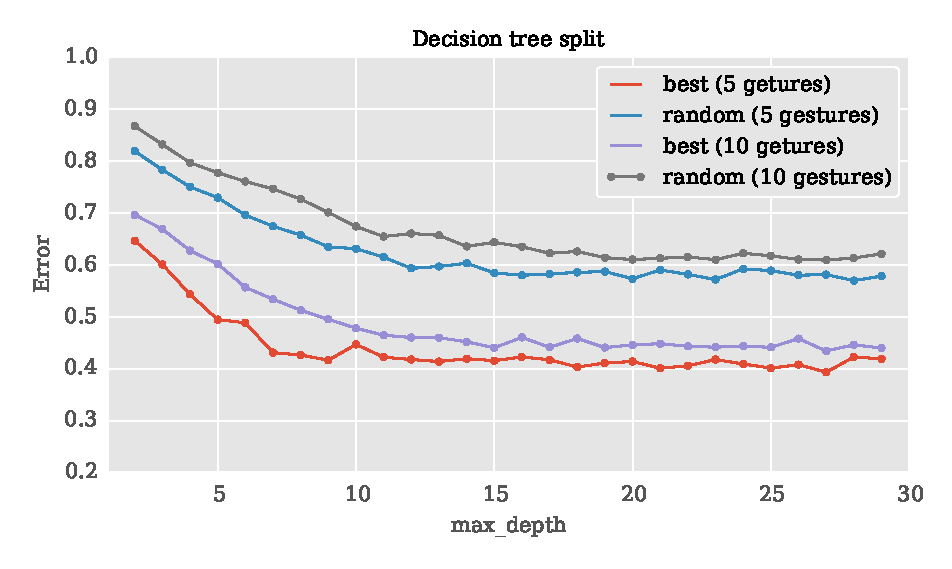
\includegraphics[width=\columnwidth]{DT_max_depth_split.eps}}
\caption{Decision tree performance for split strategies: best and random, with different maximum depth. Results is shown for $5$ gestures and $10$ gestures data sets.}
\label{fig:DT_dept_split}
\end{center}
\vskip -0.2in
\end{figure}

% ***** Random Forest  *****
\begin{figure}[t]
\vskip 0.2in
\begin{center}
\centerline{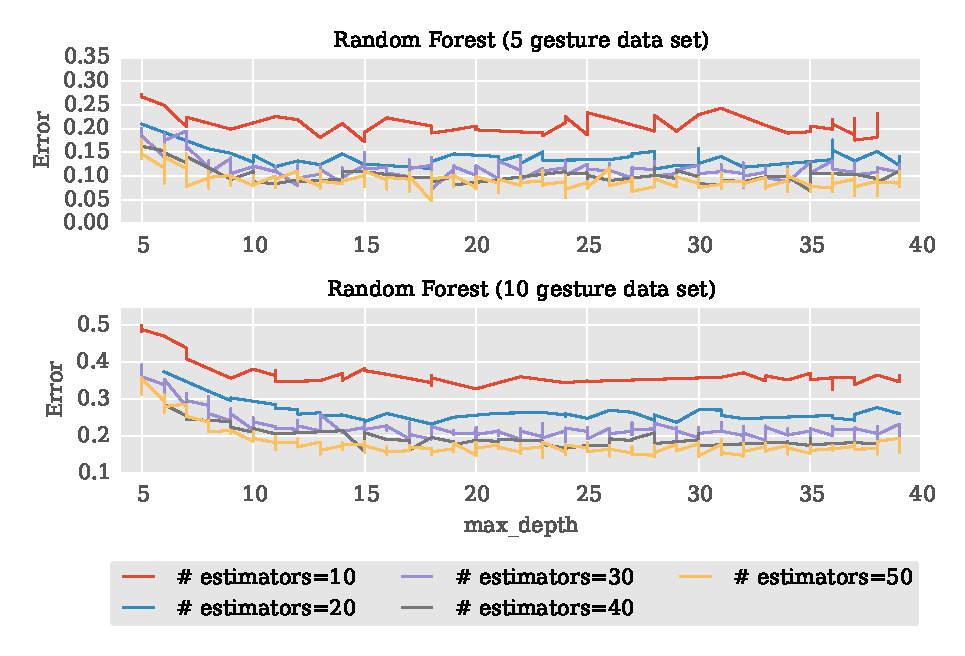
\includegraphics[width=\columnwidth]{randomForest_estimators.eps}}
\caption{Random forest performance for different number of estimators. split strategies (best and random), and for different maximum depth. Result is shown for $5$ gestures and $10$ gestures data sets.}
\label{fig:randomForest_estimators}
\end{center}
\vskip -0.2in
\end{figure}

\subsubsection{Best Models Comparison}

We compare the best models configuration of each method for the two data sets: $5$ gestures and $10$ gestures chosen by hyperopt optimization. Table~\ref{tab:bestParams} shows the best parameter values achieved by the hyper-parameter optimization algorithm. SVM and Neural networks performed better than Decision tree and Random forest as can be seen in Figure~\ref{fig:allModels_comparison}.


% ***** fig best models bar chart *****
% \begin{figure}[th]  % to position the table in the middle of the page
\begin{figure}[t]
\vskip 0.2in
\begin{center}
\centerline{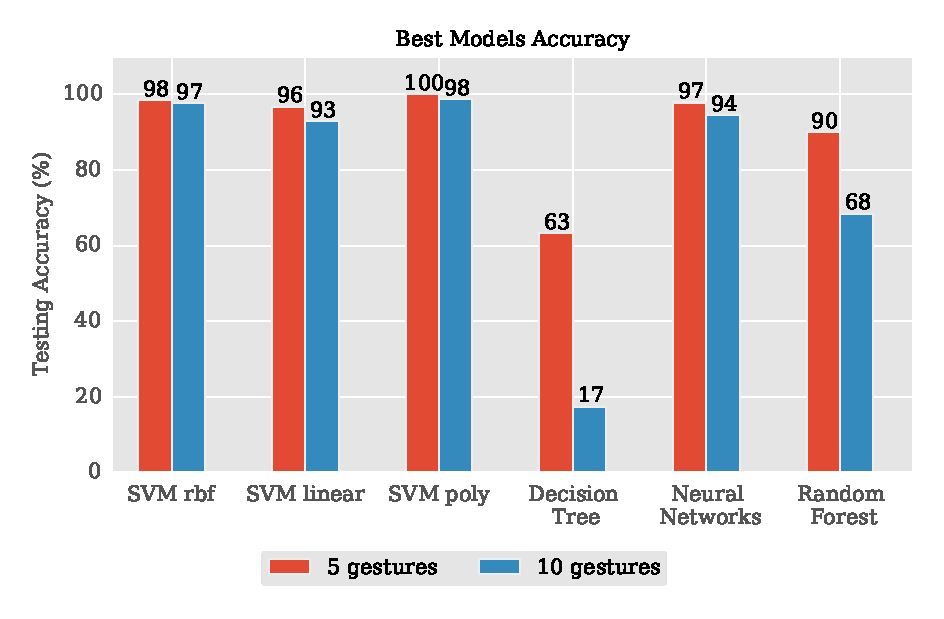
\includegraphics[width=\columnwidth]{allModels_comparison.eps}}
\caption{Comparison of the best parameters for each model.}
\label{fig:allModels_comparison}
\end{center}
\vskip -0.2in
\end{figure}

%---------------------------------------------------------------------------%
% 								End: Hossam									%
% --------------------------------------------------------------------------%
\section{Conclusion}

\bibliography{main}
\bibliographystyle{icml2015}

\end{document}

